\begin{solution}
%\begin{figure}[htbp]
\begin{center}
	%\centering
		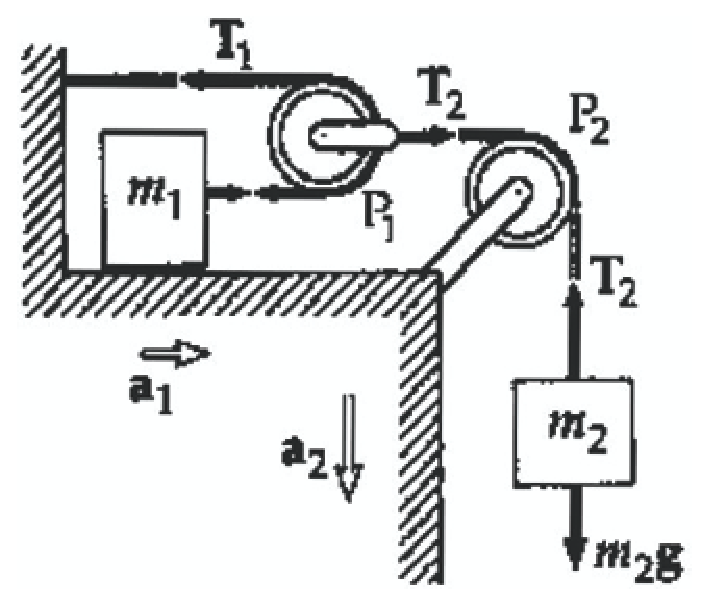
\includegraphics[scale=0.4]{./latex/eps/1_5_1_image_2.eps}
		%\caption{Gaya yang bekerja pada katrol}
	%\label{fig:1_5_1_image_2 copy}
%\end{figure}
\end{center}

a$)$Lihat gambar 2, katrol $P_{1}$ dan balok $m_{2}$ bergerak dengan percepatan $a_{2}$.
Karena balok $m_{1}$ bergerak dengan jarak 2 kali lipat dari jarak katrol $P_{1}$, maka balok $m_{1}$ mempunyai percepatan 2 kali lipat dari percepatan katrol $P_{1}$, maka $a_{1}=2 a_{2}$

b$)$ Berdasarkan hukum Newton($\Sigma F=ma$), maka gaya-gaya yang bekerja pada balok $m_{2}$, $m_{1}$, dan katrol $P_{1}$ berturur-turut adalah
\begin{eqnarray}
	m_{2}g-T_{2}=m_{2}a_{2} \\
	T_{1}=m_{1}a_{1}=2 m_{1}a_{2}\\
	T_{2}-2T_{1}=0
\end{eqnarray}
Substitusi $T_{2}$ dari persamaan 3 ke persamaan 1 menjadi $m_{2}g-2T_{1}=m_{2}a_{2} $. Persamaan ini dapat dikombinasikan dengan persamaan 2, menjadi
\begin{eqnarray*}
\frac{T_{1}}{m_{1}}\left( 2m_{1}+\frac{m_{2}}{2} \right)=m_{2}g \\
T_{1}=\frac{m_{1}m_{2}}{2 m_{1}+\frac{1}{2}m_{2}}g \quad \mbox{dan} \quad T_{2}=\frac{m_{1}m_{2}}{ m_{1}+\frac{1}{4}m_{2}}g
\end{eqnarray*}

c$)$ Setelah mengetahui nilai $T_{1}$ dan $T_{2}$, percepatan dapat dicari dengan menggunakan persamaan 2 
\begin{eqnarray*}
a_{1}=\frac{T_{1}}{m_{1}}=\frac{m_{2} g}{2 m_{1}+\frac{1}{2} m_{2}} \\
a_{2}=\frac{1}{2}a_{1}=\frac{m_{2}g}{4 m_{1+m_{2}}}
\end{eqnarray*}
\end{solution}
